\section{Evaluation}\label{sec:experiment}

\subsection{Experimental setting}

\paragraph{Datasets} We evaluate the explainability methods on both synthetic and real-world datasets in different domains, including MUTAG, BBBP, MNIST, BA-2Motifs and BA-MultiShapes. \textbf{BA-2Motifs}~\cite{PGExplainer} is a synthetic dataset with binary graph labels. The house motif and the cycle motif give class labels and thus are regarded as ground-truth explanations for the two classes. \textbf{BA-MultiShapes}~\cite{bamultishapes} is a more complicated synthetic dataset with multiple motifs. Class 0 indicates that the instance is a plain BA graph or a BA graph with a house, a grid, a wheel, or the three motifs together. On the contrary, Class 1 denotes BA graphs with two of these three motifs. \textbf{MUTAG} is a collection of $\sim$3000 nitroaromatic compounds and it includes binary labels on their mutagenicity on Salmonella typhimurium. The chemical fragments -NO2 and -NH2 in mutagen graphs are labeled as ground-truth explanations~\cite{PGExplainer}. The Blood–brain barrier penetration \textbf{BBBP} dataset includes binary labels for over 2000 compounds on their permeability properties. In molecular datasets, node features encode the atom type and edge features encode the type of bonds that connect atoms. \textbf{MNIST75sp} contains graphs that are converted from images in MNIST~\cite{lecun1998gradient} using superpixels. In these graphs, the nodes represent the superpixels, and the edges are determined by the spatial proximity between the superpixels. The coordinates and intensity of the corresponding superpixel construct the node features. Dataset statistics are summarized in Table~\ref{tab:dataset_performance}.

% We evaluate the explainability methods on molecular datasets, Mutag~\cite{debnath1991structure} and BBBP~\cite{wu2018moleculenet}, and on the synthetic dataset BA-2Motifs~\cite{PGExplainer}. \textbf{Mutag} is a collection of 3000 nitroaromatic compounds and it includes binary labels on their mutagenicity on Salmonella typhimurium. The chemical fragments -NO2 and -NH2 in mutagen graphs are labeled as ground-truth explanations~\cite{PGExplainer}. The Blood–brain barrier penetration \textbf{BBBP} dataset includes binary labels for over 2000 compounds on their permeability properties. In molecular datasets, node features encode the atom type and edge features encode the type of bonds that connect atoms. \textbf{BA-2Motifs} is a synthetic dataset with binary graph labels. The house motif and the cycle motif give class labels and thus are regarded as ground-truth explanations for the two classes.

% All experiments are conducted on a Linux machine with an Nvidia GeForce RTX 2070 SUPER GPU with 8GB memory. CUDA version is 11.1. Methods are implemented with Torch 1.9.1.

\begin{table}[ht]
\centering
\resizebox{0.8\linewidth}{!}{
\begin{tabular}{lccc||cc}
\toprule
                 & \textbf{MUTAG} & \textbf{BBBP} & \textbf{MNIST75sp}  & \textbf{BA-2Motifs} & \textbf{BA-MultiShapes}\\ \hline
\# graphs        & 2,951  & 2,039 & 70,000 & 1,000 &  1,000    \\ 
\# node features & 14    & 9    & 5      & 1    &   10    \\ 
\# edge features & 1     & 3    & 1      & 1    &   1   \\ 
Avg \# nodes     & 30  & 24 & 67     & 25   &    40  \\ 
Avg \# edges     & 61    & 52   & 541    & 51   &     87  \\ 
Avg degree       & 2.0     & 2.1  & 7.9    & 2.0    &    2.2   \\ 
\# classes       & 2     & 2    & 10     & 2    &   2   \\ 
GNN performance  & 0.94      &  0.92    &  0.96      &  1.00    &   0.71    \\
\bottomrule
\end{tabular}}
\caption{Dataset statistics and accuracy performance of the GNN model on the test set}\label{tab:dataset_performance}
\end{table}
\paragraph{GNN models}  For each dataset, we first train a GNN model. We have tested four GNN models: GCN \cite{GCN}, GIN\cite{GIN}, GAT \cite{GAT}, and GraphTransformer \cite{GraphTransf}. We only display results for the GraphTransformer model for the real-world datasets and the GIN model for the synthetic datasets since they give the highest accuracy scores on the test sets respectively. GraphTransformer and GIN give high accuracy on the real-world and synthetic datasets respectively, with a reasonable training time and fast convergence. Unlike GCN, GraphTransformer and GIN have also the advantage of taking edge features, extending their use to more complex graph datasets. The network structure of the GNN model for graph classification is a series of 3 layers with ReLU activation, followed by a max pooling layer to get graph representations before the final fully connected layer. We adopt the Adam optimizer with an initial learning rate of 0.001. We split train/validation/test with 80/10/10$\%$ for all datasets. Each model is trained for 200 epochs with an early stop. The accuracy performances of GNN models are shown in Table~\ref{tab:dataset_performance}. The results show that the designed GNN models are sufficiently powerful for graph classifications on both synthetic and real-life datasets.

\paragraph{Explainability methods} We compare non-generative methods: Saliency~\cite{SA-Graph}, Integrated Gradient~\cite{IG}, Occlusion~\cite{occlusion}, Grad-CAM~\cite{Grad-CAM-Graph}, GNNExplainer~\cite{GNNExplainer}, PGMExplainer~\cite{PGM-Explainer}, and SubgraphX~\cite{SubgraphX}, with generative ones: PGExplainer~\cite{PGExplainer}, GSAT~\cite{GSAT}, GraphCFE (CLEAR)~\cite{CLEAR}, D4Explainer and RCExplainer~\cite{RCExplainer}. Following GraphFramEx~\cite{GraphFramEx}, we define an explanation as an edge mask on the existing edges in the initial graph to be explained. First, this constraint facilitates the comparison of very diverse explainability methods. Moreover, in the context of our study, all datasets are expected to be explained by some entities that already exist in the initial graphs, \ie motifs in synthetic datasets and groups of atoms in molecular datasets. We follow the original setting to train PGExplainer, GSAT, and RCExplainer. We implement the diffusion-based explainer as introduced in Sec.~\ref{sec:generative_model}, and name it D4Explainer. D4Explainer generates an explanatory graph that can contain additional edges that are not in the initial graph. To keep consistent, we retrieve the common edges with the initial graph to evaluate D4Explainer in this work. GraphCFE is a simplified version of CLEAR~\cite{CLEAR} without the causality component, which is an explainability method for counterfactual explanations. Indeed, the causal models introduced in~\cite{CLEAR} are constructed from simulations because it is hard to get the ground-truth causal model from datasets. Since we ignore the existence of any causal model in our datasets, we decide not to focus on the causality and use only the CLEAR-VAE backbone, \ie GraphCFE, in this work. We retrieve the important edges by subtracting the counterfactual explanation generated by GraphCFE from the initial graph. The remaining edges have weights of 1, while the rest have weights of 0.



% \textbf{PGExplainer}~\cite{PGExplainer} trains an additional neural network that takes as input the edge features and outputs an edge weight for each edge in the initial graph. We restrict the edge weight in the range of $[0,1]$ and create an explanation mask for the initial graph. \textbf{GSAT}~\cite{GSAT} method generates explanatory subgraphs by learning stochastic attention parameters learned from a Bernoulli distribution that drop the edges in the initial graph. The explanatory edge mask is the attention coefficient for each edge of the initial graph computed by the train GSAT. The diffusion-based explainability method \textbf{D4Explainer} generates an explanatory graph that can contain additional edges that are not in the initial graph. For a fair comparison, we retrieve the common edges with the initial graph to evaluate D4Explainer in this work. The explanatory edge mask corresponds to the weights of the common edges. \textbf{RCExplainer}~\cite{RCExplainer} is a reinforcement learning based explainer. It indicates which edge should be added in the next step during the sequential generation process. From this sequential generation order, we can retrieve a ranking from the most important edges to the least important ones. We compute the importance of each edge $i$ as $w_i = 1-\textsc{rank}(i)/|E|$. The edge mask is the list of these weights ranging from 0 to 1. \textbf{GraphCFE} is a simplified version of CLEAR~\cite{CLEAR} without the causality component, which is an explainability method for counterfactual explanations. Indeed, the causal models introduced in~\cite{CLEAR} are constructed from simulations because it is hard to get the ground-truth causal model from datasets. Since we ignore the existence of any causal model in our datasets, we decide not to focus on the causality and use only the CLEAR-VAE backbone, \ie GraphCFE. We retrieve the important edges by subtracting the counterfactual explanation generated by GraphCFE from the initial graph. The remaining edges have weights of 1, while the rest have weights of 0.

% \textbf{GFlowExplainer}~\cite{GFlowExplainer} is also an RL-based method. Once trained, it gives the order of edges to be removed from the initial graph in order to preserve the highest reward. From this removal ranking, we construct the edge mask as the list of weights $i = rank_r(i)/|E|$ where $rank_r$ denotes the removal rank.

\paragraph{Metrics} To evaluate the explainability methods, we use the systematic evaluation framework GraphFramEx~\cite{GraphFramEx}. We evaluate the methods on the faithfulness measure $fidelity-_{acc}$, which is defined as
$$fidelity-_{acc}= \frac{1}{N} \sum_{i=1}^{N}\left| \mathbbm{1}(\hat{Y}_f(G^i)=Y^i)- \mathbbm{1}(\hat{Y}_f(G^i_e)=Y^i) \right|,$$
where $G^i$ and $G^i_e$ denote the initial graph and the explanatory graph, respectively. $fidelity-_{acc}$ measures if the generated explanatory subgraph is faithful to the initial graph, \ie leads to the same GNN prediction. 
\subsection{Instance-level explanations}
\paragraph{Faithfulness} We conducted a comprehensive comparison of the faithfulness between generative and non-generative methods using three real-world datasets (BBBP, MUTAG, and MNIST) and two synthetic datasets (BA-2Motifs and BA-MultiShapes). The results, depicted in Figure~\ref{fig:faithfulness}, indicate that generative methods are generally performing the same or better than non-generative methods. Specifically, for MNIST, generative methods outperform non-generative methods across the board. In the cases of MUTAG and BA-2Motifs, the generative methods RCExplainer, GraphCFE, and GSAT closely follow Grad-CAM and Occlusion in terms of faithfulness. Regarding BBBP and BA-MultiShapes, both generative and non-generative methods exhibit similar results. Consequently, generative methods achieve state-of-the-art performance on benchmark graph datasets. Furthermore, we demonstrate that generative methods possess additional desirable properties, such as efficiency and generalization capacity, which make them more appealing than non-generative methods.
\begin{figure}[h!]
    \centering
    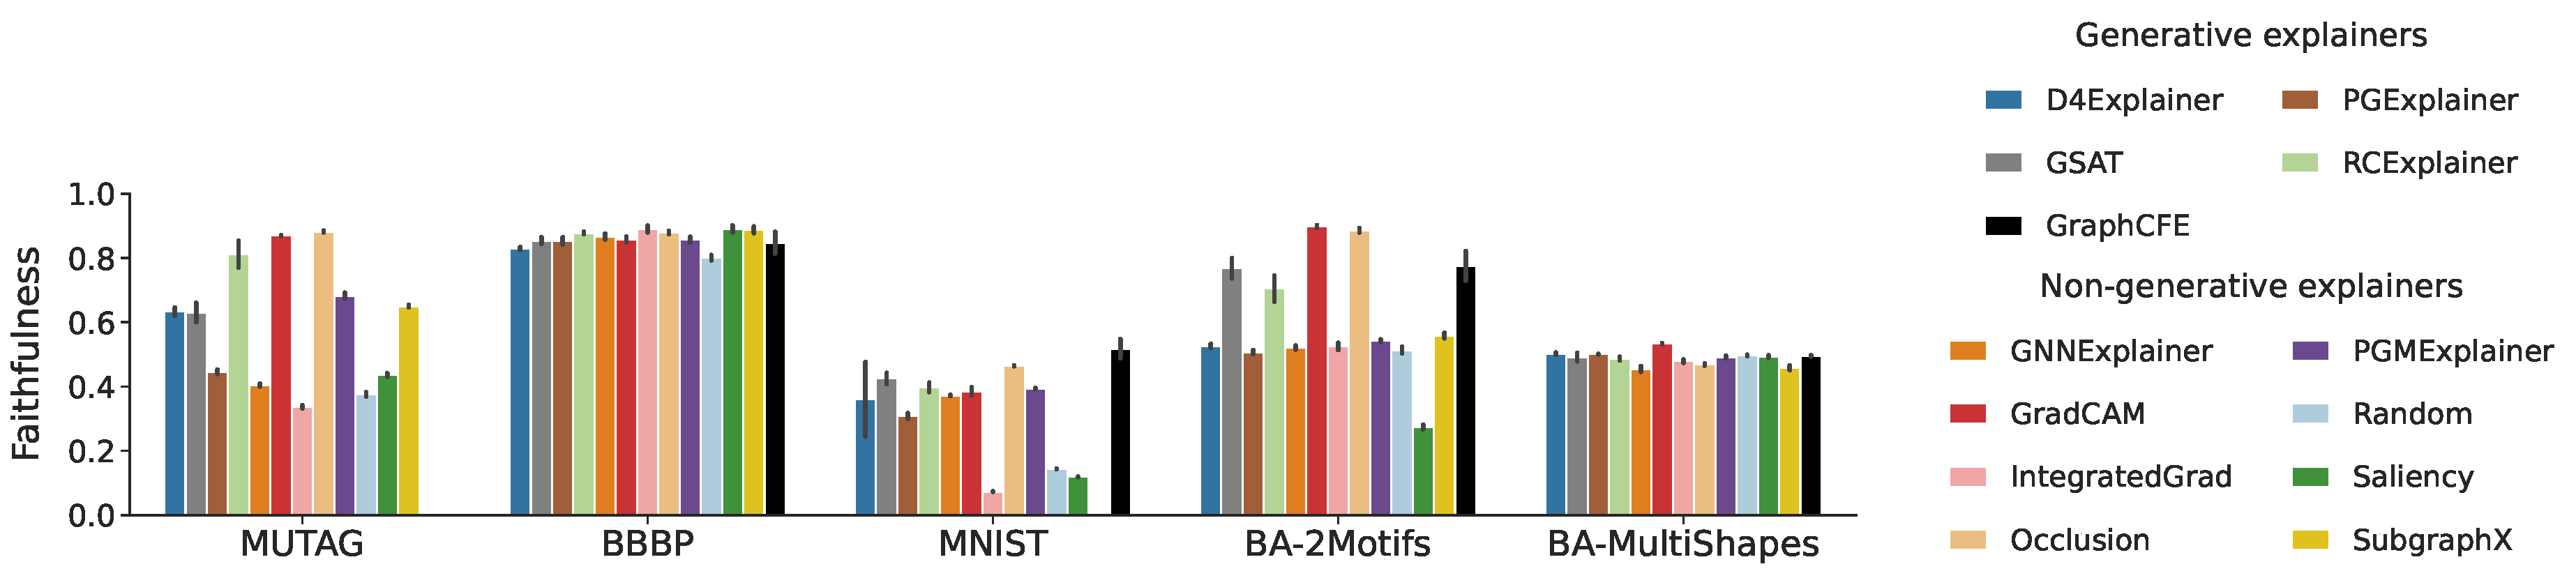
\includegraphics[width=0.85\textwidth]{submissions/Rex2023/figures/faithfulness-_5_D4.pdf}
    \caption{Faithfulness of explainability methods. On the y-axis, we report the faithfulness computed as $1-fidelity-_{acc}$. On the x-axis, generative methods are always on the left-hand side of the methods (the bars). If the score is close to 1, the explanation is very faithful. The score is averaged over all explanations with less than 20 edges to enforce sparse and human-intelligible explanations.}
    \label{fig:faithfulness}
\end{figure}
\paragraph{Efficiency} To measure the efficiency of explainability methods, we report the computation time to produce an explanation for a new instance in Figure~\ref{fig:efficiency}. Comparing generative methods with other learnable methods (\eg GNNExplainer, PGMExplainer) in Figure~\ref{fig:efficiency}, we observe that once the model is trained, generative explainability methods require shorter inference time than non-generative ones in general. The time is reported in logarithmic scale and generative methods always have inference times of the order of $10^0$ or less, except for the case of RCExplainer for MNIST. The advantage of shorter inference time is especially pronounced on large-scale datasets, \eg MNIST. We also report the time required to train a generative model from scratch in Table~\ref{tab:train_time}. 
\begin{figure}[h!]
    \centering
    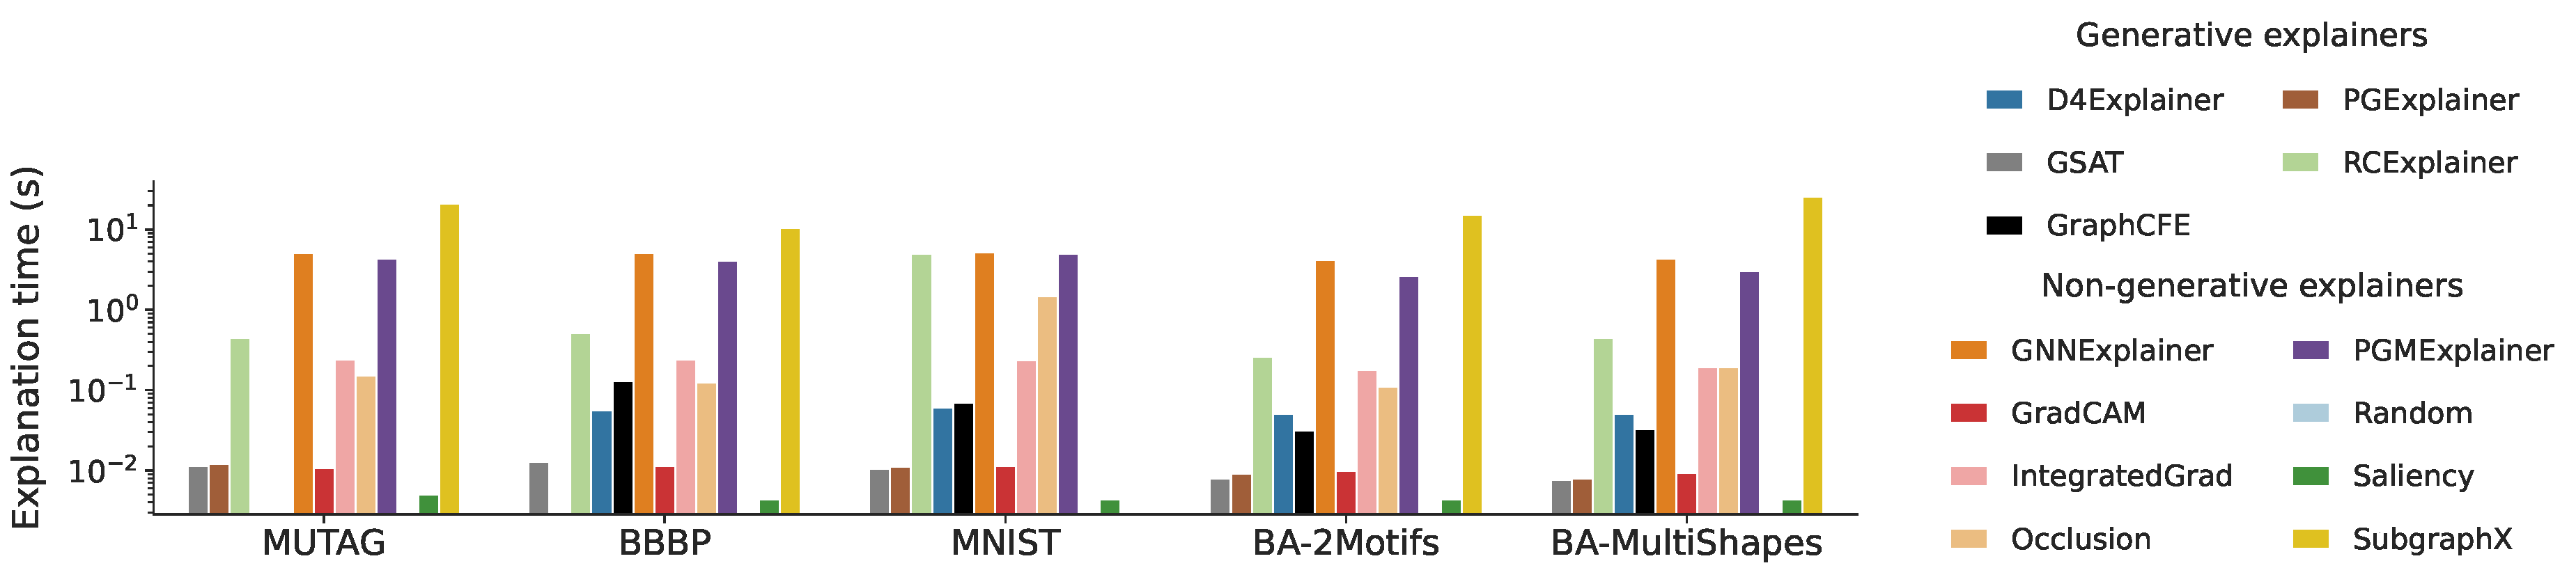
\includegraphics[width=0.75\textwidth]{submissions/Rex2023/figures/inference_time_bar_log.pdf}
    \caption{Inference time of explainability methods to explain one single graph. The computation time is averaged over 100 explanations over 5 seeds and reported in logarithmic scale.}
    \label{fig:efficiency}
\end{figure}
% We report computation times both on CPUs (8 AMD EPYC 7742 CPUs with a memory of 5GB each) and on GPU (Nvidia GeForce RTX 2070 SUPER GPU with 8GB memory).
\begin{table}[h]
\centering
\resizebox{0.8\linewidth}{!}{
\begin{tabular}{l|ccccc}
 & \textbf{D4Explainer} & \textbf{GraphCFE} & \textbf{GSAT} & \textbf{PGExplainer} & \textbf{RCExplainer} \\ \hline
\textbf{BA-2Motifs} & 475.3                  & 320.9             & 23.1          & 11.6                 & 194.0                \\ 
\textbf{BA-MultiShapes} & 309.3                  & 211.8             & 20.0          & 17.2                 & 251.0                \\ 
\textbf{BBBP}       & 385.6                  & 1350.0            & -             & 26.0                 & 303.4                \\ 
\textbf{MNIST}      & 934.6                  & 929.5             & 41.4          & 28.6                 & 3271.0               \\ 
\textbf{MUTAG}      & 253.1                  & -                 & 79.8          & 27.7                 & 434.6                \\ \hline
Mean                & 471.6                  & 703.1             & 41.1         & 22.2                 & 890.8               \\ 
\end{tabular}}
\caption{Training times (s) of the generative methods with 1 GPU (Nvidia GeForce RTX 2080)}
\label{tab:train_time}
\end{table}
\begin{figure}[h]
    \centering
    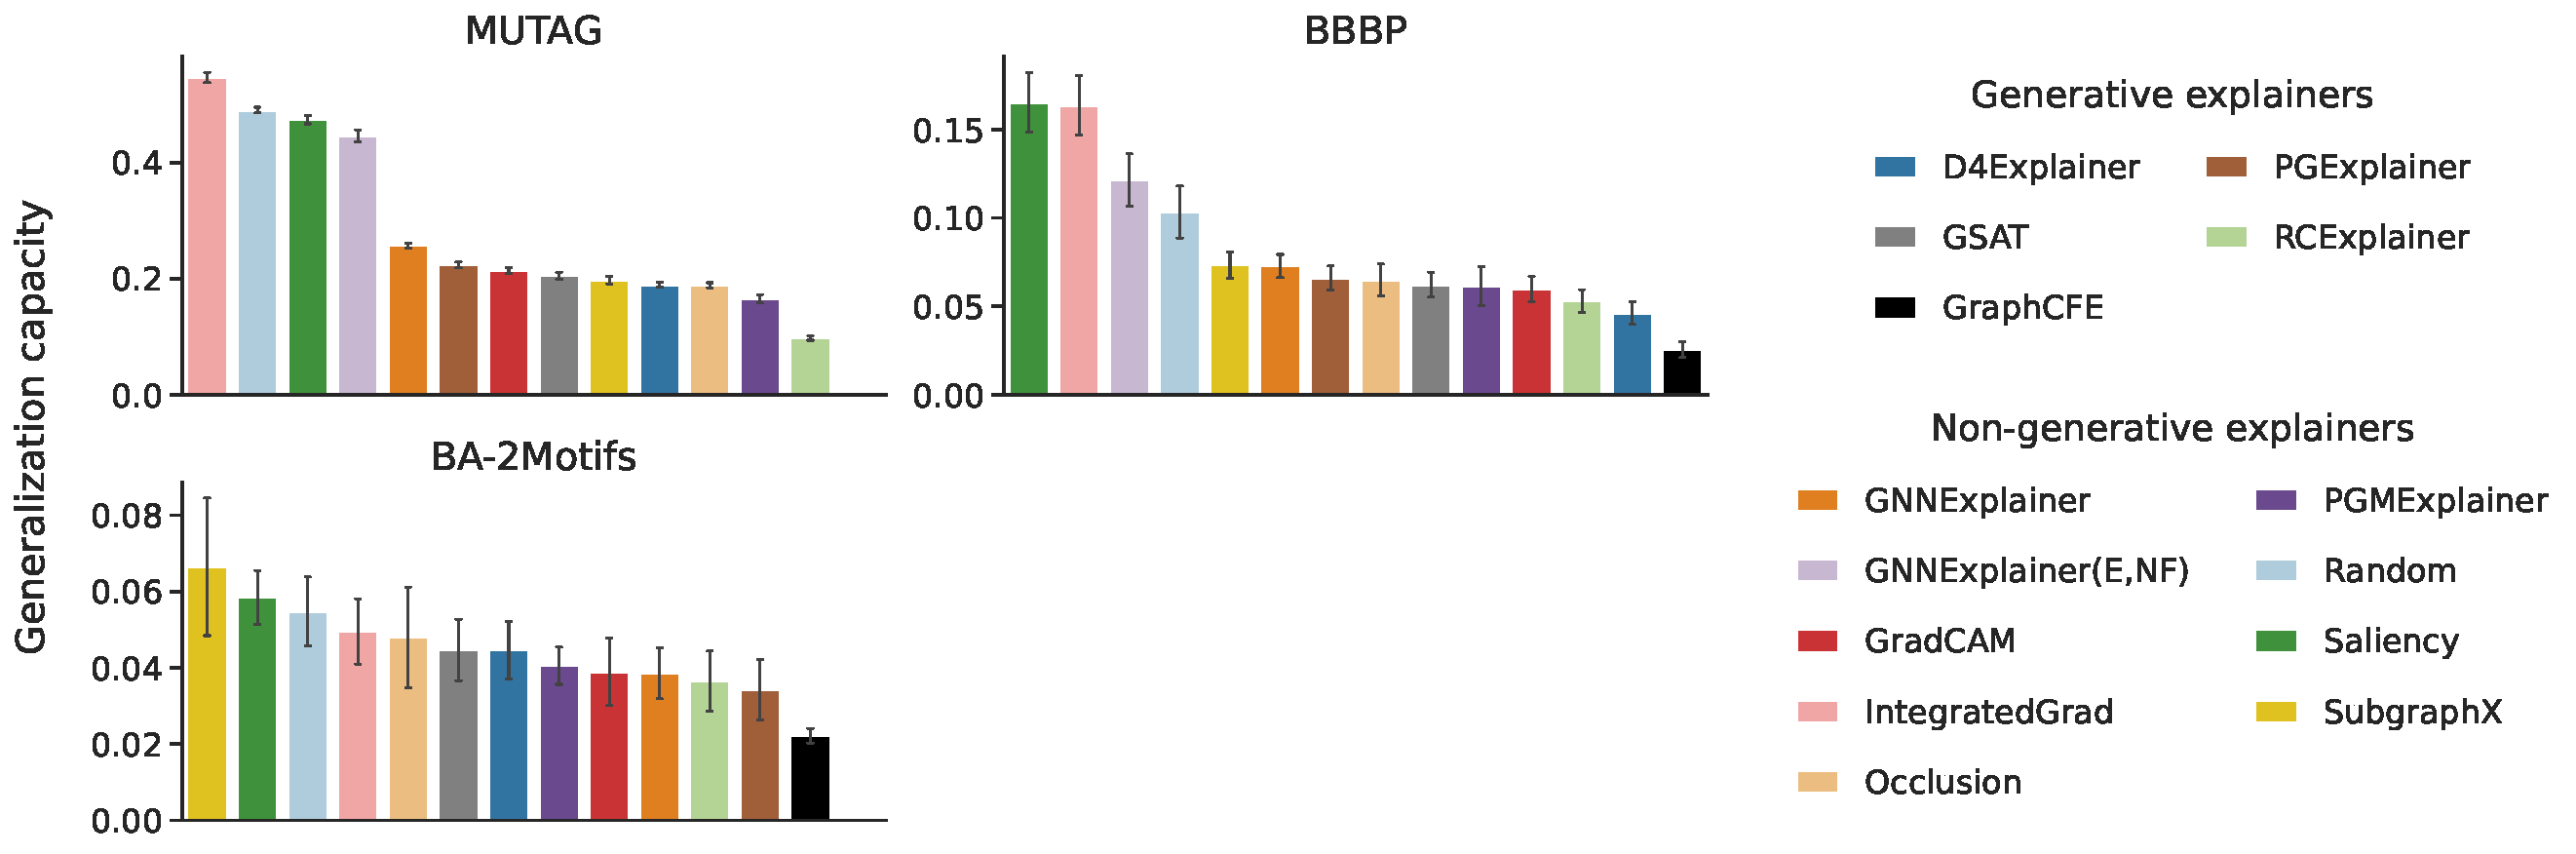
\includegraphics[width=0.75\textwidth]{submissions/Rex2023/figures/gen_capacity_3.pdf}
    \caption{Generalization capacity of explainability methods is computed by subtracting the performance on data seen during training and the performance on unseen data. The lower the discrepancy reported on the y-axis, the better the method can generalize to unseen data. GNNExplainer indicates the explanations at only edge-level and GNNExplainer(E,NF) represents the explanations for both edges and node features.}
    \label{fig:generalization}
\end{figure}
\paragraph{Generalization} To compare generative and non-generative explainability methods on their generalization capacity, we split the datasets into seen and unseen data. The split ratio is 90/10$\%$. We further split the seen data into training, validation, and test set. The GNN model and the generative explainability methods are trained on the seen data. For non-generative methods, we explain 100 graphs from the seen dataset. Then, we test the trained methods on the unseen data. In Figure~\ref{fig:generalization}, we report the scores discrepancies between the test set of the seen data and the 10$\%$ unseen data for each explainability method. We also visualize the standard error on the five random seeds in Figure~\ref{fig:generalization}. Methods with higher absolute score discrepancies cannot generalize well to unseen data, while the ones with lower score discrepancies have a powerful generalization capacity. We can observe from Figure~\ref{fig:generalization} that generative explainability methods have lower scores than non-generative methods across three datasets in general, which demonstrates the better generalization capacity.


% \begin{figure}
%     \centering
%     \includegraphics[width=0.75\textwidth]{submissions/Rex2023/figures/top_balanced_acc_syn.pdf}
%     \caption{Caption}
%     \label{fig:top_acc_syn}
% \end{figure}

% \begin{figure}
%     \centering
%     \includegraphics[width=0.85\textwidth]{submissions/Rex2023/figures/fid+fid-acc.pdf}
%     \caption{Caption}
%     \label{fig:fid+/-}
% \end{figure}

% \begin{figure}
%     \centering
%     \includegraphics[width=0.85\textwidth]{submissions/Rex2023/figures/charact_acc.pdf}
%     \caption{Caption}
%     \label{fig:charact_topk}
% \end{figure}

% \subsection{Counterfactual explanations}


